\documentclass[11pt,a4paper]{article}

\usepackage[utf8]{inputenc}
\usepackage[T1]{fontenc}
\usepackage[margin=1in]{geometry}
\usepackage{amsmath,amssymb}
\usepackage{graphicx}

\newtheorem{theorem}{Theorem}
\newtheorem{lemma}{Lemma}
\newenvironment{proof}{\par\noindent\textit{Proof.}\ }{\hfill$\square$\par\medskip}

\title{\textbf{Distributionally-Robust Cloud Capacity Scaling and Correlated Spot Portfolio Optimization via Adaptive Conformal Inference and CVaR MILP}}

\author{
  Abdelrahman H. Farag \\
  Independent Systems \& Applied Mathematics Research \\
  \texttt{https://github.com/ahafarag/aegis-scale}
}

\date{November 2026}

\begin{document}
\sloppy
\maketitle

\begin{abstract}
Cloud infrastructure operators face a persistent trade-off between compute expenditure and service-level agreement (SLA) continuity. Provisioning exclusively On-Demand virtual machines guarantees capacity availability at a $2.5\times$--$5\times$ cost premium, whereas greedy adoption of discounted Spot instances exposes services to correlated capacity recalls across Availability Zones (AZs) and processor families, causing severe tail-latency ($\mathrm{P99}$) violations during non-stationary traffic bursts. We introduce \textsc{AegisScale}, a three-layer mathematical control architecture that unifies distribution-free online statistical learning, heavy-traffic queueing diffusion bounds, and risk-averse discrete optimization. First, Adaptive Conformal Inference (ACI) wraps a scale-invariant harmonic-autoregressive Recursive Least Squares (RLS) filter to provide finite-sample demand coverage bounds without distributional or stationarity assumptions. Second, a Kingman--Sakasegawa $G/G/c$ heavy-traffic queueing mapping translates conformal arrival-rate envelopes into exact minimum safe vCPU requirements satisfying $\mathrm{P99}$ queueing delay constraints while reducing analytically to the exact $M/M/1$ waiting-time quantile at $c=1$. Third, a three-factor Gaussian hazard copula generates correlated $(\text{AZ}, \text{family})$ Spot preemption scenarios for an auxiliary-free Rockafellar--Uryasev Conditional Value-at-Risk ($\mathrm{CVaR}_\beta$) Mixed-Integer Linear Program (MILP) solved globally via HiGHS. Evaluated across both a 7-day multi-storm synthetic benchmark and 4,032 production intervals (14 days) of real AWS CloudWatch Elastic Load Balancer telemetry, \textsc{AegisScale} reduces annualized compute spend by $35.7\%$--$38.7\%$ compared to equal-SLA On-Demand provisioning while sustaining $>99.5\%$ $\mathrm{P99}$ SLA continuity, empirical conformal miscoverage of $1.488\%$ (target $1.500\%$), $\sim 46.8\,\mathrm{ms}$ median solve latency, and zero correlated Spot-storm outages.
\end{abstract}

\section{Introduction}

Modern cloud-native workloads operate over heterogeneous compute markets in which providers sell identical physical silicon under two contrasting contracts: guaranteed \emph{On-Demand} capacity at fixed hourly rates, and revocable \emph{Spot} capacity discounted by $60\%$--$85\%$ subject to two-minute preemption warnings. Standard reactive autoscalers---such as Kubernetes Horizontal Pod Autoscaler (HPA) or AWS Auto Scaling Target Tracking---scale capacity only after utilization metrics breach static thresholds (typically $50\%$--$60\%$ CPU). Under non-stationary flash crowds or correlated regional Spot recalls, reactive controllers suffer queueing instability, whereas static Spot heuristics fail to account for cross-pool correlation across Availability Zones and CPU families.

\textsc{AegisScale} resolves these limitations through three verifiable mathematical contributions:
\begin{enumerate}
    \item \textbf{Distribution-Free Online Demand Envelopes:} We pair a scale-invariant delta-harmonic Recursive Least Squares filter with Gibbs and Cand\`es' Adaptive Conformal Inference~\cite{gibbs2021adaptive}, proving deterministic finite-sample miscoverage bounds on arbitrary bounded workload sequences (Theorem~\ref{thm:aci}).
    \item \textbf{Exact $M/M/1$-Consistent $G/G/c$ Tail Sizing:} Combining Sakasegawa's delay probability~\cite{sakasegawa1977approximation} with Kingman's heavy-traffic exponential waiting law~\cite{kingman1961single,whitt1993approximations}, we establish strict monotonicity and exact $M/M/1$ closed-form equivalence (Lemma~\ref{lem:ggc}), enabling machine-precision capacity bisection in $O(\log(1/\epsilon))$ evaluations.
    \item \textbf{Auxiliary-Free Non-Negative Shortfall $\mathrm{CVaR}_\beta$ MILP:} Using a three-factor Gaussian copula~\cite{li2000default} with antithetic variance reduction, we prove that constraining the Rockafellar--Uryasev threshold $\eta \ge 0$ linearizes non-negative capacity shortfall $\max(0, C_{\mathrm{req}} - C_{\mathrm{surv}})$ without $S$ intermediate slack variables (Lemma~\ref{lem:cvar}), enabling real-time global integer solutions via HiGHS~\cite{huangfu2018parallelizing}.
\end{enumerate}

\section{Mathematical Formulation}

\subsection{Layer 1: Scale-Invariant RLS and Adaptive Conformal Inference}

Let $\{D_t\}_{t=1}^T \subset \mathbb{R}_{\ge 0}$ denote observed request arrival rates (requests/sec) over discrete control intervals. Maintaining an exponentially weighted running scale $\sigma_t = 0.95\sigma_{t-1} + 0.05\max(1, D_t)$, we model normalized increments $\Delta_t = (D_t - D_{t-1})/\sigma_{t-1}$ via feature vector
\begin{equation}
    \phi_t = \left[1, \; \Delta_{t-p}, \dots, \Delta_{t-1}, \; \sin\!\left(\frac{2\pi t}{P}\right), \cos\!\left(\frac{2\pi t}{P}\right), \sin\!\left(\frac{4\pi t}{P}\right), \cos\!\left(\frac{4\pi t}{P}\right)\right]^\top \in \mathbb{R}^{p+5},
\end{equation}
updated online via forgetting-factor RLS ($\lambda_{\mathrm{rls}} = 0.985$) in $O((p+5)^2)$ arithmetic operations per step, yielding one-step point forecast $\hat{D}_{t|t-1} = \max(0, D_{t-1} + \sigma_{t-1}\,\mathrm{clip}(\theta_{t-1}^\top \phi_t, -0.75, 0.75))$.

Let $r_i = D_i - \hat{D}_{i|i-1}$ denote signed conformity residuals in a sliding calibration window $\mathcal{W}_t$ of size $W$. Define the empirical quantile $\hat{Q}_{1-\alpha}(\mathcal{W}_t)$ at level $1-\alpha$, with boundary conventions $\hat{Q}_{1-\alpha} = +\infty$ for $\alpha \le 0$ and $\hat{Q}_{1-\alpha} = -\infty$ for $\alpha \ge 1$. Setting upper demand envelope $\hat{U}_t(\alpha_t) = \hat{D}_{t|t-1} + \hat{Q}_{1-\alpha_t}(\mathcal{W}_t)$ and indicator $\mathrm{err}_t = \mathbb{I}\{D_t > \hat{U}_t(\alpha_t)\}$, we evolve the unclipped dual state:
\begin{equation}\label{eq:aci}
    \alpha_{t+1} = \alpha_t + \gamma(\alpha_{\mathrm{target}} - \mathrm{err}_t), \qquad \gamma > 0, \; \alpha_1 = \alpha_{\mathrm{target}} \in (0, 1).
\end{equation}

\begin{theorem}[Finite-Sample Non-Stationary Coverage]\label{thm:aci}
For any bounded deterministic or adversarial workload sequence $\{D_t\}_{t=1}^T$, the dual iterate~\eqref{eq:aci} satisfies $\alpha_t \in [-\gamma, 1 + \gamma]$ for all $t \ge 1$, and the empirical demand under-provisioning frequency obeys
\begin{equation}
    \left| \frac{1}{T}\sum_{t=1}^T \mathrm{err}_t - \alpha_{\mathrm{target}} \right| \le \frac{1 + 2\gamma}{\gamma T}.
\end{equation}
\end{theorem}
\begin{proof}
Whenever $\alpha_t \le 0$, $\hat{U}_t(\alpha_t) = +\infty \implies \mathrm{err}_t = 0$, giving $\alpha_{t+1} = \alpha_t + \gamma\alpha_{\mathrm{target}} > \alpha_t$; because any single step decreases $\alpha$ by at most $\gamma(1-\alpha_{\mathrm{target}}) < \gamma$, induction yields $\alpha_t \ge -\gamma$. Symmetrically, whenever $\alpha_t \ge 1$, $\hat{U}_t(\alpha_t) = -\infty \implies \mathrm{err}_t = 1$, giving $\alpha_{t+1} = \alpha_t - \gamma(1-\alpha_{\mathrm{target}}) < \alpha_t$ and hence $\alpha_t \le 1 + \gamma$. Summing~\eqref{eq:aci} over $t=1,\dots,T$ telescopes to $\alpha_{T+1} - \alpha_1 = \gamma\sum_{t=1}^T (\alpha_{\mathrm{target}} - \mathrm{err}_t)$. Dividing by $\gamma T$ and bounding $|\alpha_{T+1} - \alpha_1| \le 1 + 2\gamma$ establishes the claim.
\end{proof}

\subsection{Layer 2: Kingman--Sakasegawa $G/G/c$ Queueing Delay Sizing}

Given upper arrival rate $\hat{\lambda} = \hat{U}_t$, per-vCPU service rate $\mu > 0$, inter-arrival squared coefficient of variation $c_a^2$, and service squared coefficient of variation $c_s^2$, let $\rho(c) = \hat{\lambda}/(c\mu) < 1$ for $c > \hat{\lambda}/\mu$. Combining Sakasegawa's queueing probability $P_{\mathrm{wait}}(c) = \rho(c)^{\sqrt{2(c+1)}-1}$ with Kingman's heavy-traffic mean wait $\mathbb{E}[W_q(c)] = \frac{c_a^2 + c_s^2}{2}\frac{\rho(c)^{\sqrt{2(c+1)}-1}}{c\mu(1-\rho(c))}$, the conditional mean wait given queueing is $\mathbb{E}[W_q(c) \mid W_q > 0] = \frac{c_a^2 + c_s^2}{2c\mu(1-\rho(c))}$. Under heavy-traffic exponential tail decay, the $(1-\delta)$-quantile waiting time is
\begin{equation}\label{eq:ggc_quantile}
    W_{q, 1-\delta}(c) = \begin{cases}
        0, & P_{\mathrm{wait}}(c) \le \delta, \\[4pt]
        \left(\dfrac{c_a^2 + c_s^2}{2}\right)\dfrac{1}{c\mu(1-\rho(c))}\ln\!\left(\dfrac{P_{\mathrm{wait}}(c)}{\delta}\right), & P_{\mathrm{wait}}(c) > \delta.
    \end{cases}
\end{equation}

\begin{lemma}[Exact $M/M/1$ Reduction and Global Uniqueness]\label{lem:ggc}
At $c=1$ and $c_a^2 = c_s^2 = 1$, Eq.~\eqref{eq:ggc_quantile} reduces identically to the exact closed-form stationary $M/M/1$ waiting-time quantile $W_{q,1-\delta}(1) = \max(0, \ln(\rho/\delta)/[\mu(1-\rho)])$. Moreover, for any $c_a^2 + c_s^2 > 0$, $W_{q,1-\delta}(c)$ is continuous and strictly decreasing wherever positive on $(\hat{\lambda}/\mu, \infty)$, guaranteeing a unique root $C_{\mathrm{req}}$ to $W_{q,1-\delta}(c) \le \tau_{\mathrm{SLA}}$.
\end{lemma}
\begin{proof}
At $c=1$, $\sqrt{2(1+1)}-1 = 1$, so $P_{\mathrm{wait}}(1) = \rho$, yielding the exact $M/M/1$ quantile law. For $c > \hat{\lambda}/\mu$, $c\mu(1-\rho(c)) = c\mu - \hat{\lambda}$ is strictly increasing in $c$, while $\rho(c) \in (0, 1)$ is strictly decreasing and $\sqrt{2(c+1)}-1$ is strictly increasing, making $P_{\mathrm{wait}}(c)$ strictly decreasing. Thus $W_{q,1-\delta}(c)$ is a product of positive, continuous, strictly decreasing functions on $\{c : P_{\mathrm{wait}}(c) > \delta\}$.
\end{proof}

\subsection{Layer 3: Correlated Spot Hazard Copula and Exact CVaR MILP}

Let $\mathcal{K} = \mathcal{I}_{\mathrm{OD}} \cup \mathcal{I}_{\mathrm{Spot}}$ index $K$ compute pools with vCPUs $v_k$, hourly prices $p_k$, Availability Zones $a(k)$, and hardware families $f(k)$. Latent capacity stress in scenario $s \in \{1,\dots,S\}$ is generated via the three-factor Gaussian copula
\begin{equation}
    Z_k^{(s)} = \sqrt{\rho_{\mathrm{az}}}\,G_{a(k)}^{(s)} + \sqrt{\rho_{\mathrm{fam}}}\,H_{f(k)}^{(s)} + \sqrt{1 - \rho_{\mathrm{az}} - \rho_{\mathrm{fam}}}\,\epsilon_k^{(s)},
\end{equation}
with $\xi_k^{(s)} = \mathbb{I}\{Z_k^{(s)} < \Phi^{-1}(p_k^{\mathrm{intr}})\}$ for $k \in \mathcal{I}_{\mathrm{Spot}}$ and $\xi_k^{(s)} \equiv 0$ for $k \in \mathcal{I}_{\mathrm{OD}}$. Antithetic pairs $(G,H,\epsilon) \mapsto (-G,-H,-\epsilon)$ halve sampling variance.

For integer allocation $x \in \mathbb{Z}_{\ge 0}^K$, surviving capacity in scenario $s$ is $C_{\mathrm{surv}}^{(s)}(x) = \sum_{k=1}^K v_k(1 - \xi_k^{(s)})x_k$, signed deficit is $d_s(x) = C_{\mathrm{req}} - C_{\mathrm{surv}}^{(s)}(x)$, and actual capacity shortfall is $L_s(x) = \max(0, d_s(x)) \ge 0$.

\begin{lemma}[Auxiliary-Free Non-Negative Shortfall $\mathrm{CVaR}_\beta$ Linearization]\label{lem:cvar}
Restricting $\eta \ge 0$ in the Rockafellar--Uryasev functional~\cite{rockafellar2000optimization} yields the exact identity
\begin{equation}
    \min_{\eta \ge 0} \left\{ \eta + \frac{1}{(1-\beta)S}\sum_{s=1}^S \max\!\big(0, \; d_s(x) - \eta\big) \right\} = \mathrm{CVaR}_\beta\big(L(x)\big)
\end{equation}
without introducing $S$ auxiliary variables to represent $L_s(x) = \max(0, d_s(x))$.
\end{lemma}
\begin{proof}
Since $L_s(x) \ge 0$ for every scenario $s$, its $\beta$-quantile satisfies $\eta^* = \mathrm{VaR}_\beta(L(x)) \ge 0$. For any $\eta \ge 0$ and any $d_s \in \mathbb{R}$: if $d_s \ge 0$, $d_s = L_s$; if $d_s < 0$, then $d_s - \eta < 0$ and $L_s - \eta = -\eta \le 0$, so $\max(0, d_s - \eta) = 0 = \max(0, L_s - \eta)$.
\end{proof}

Consequently, the complete fleet allocation problem reduces to the compact MILP:
\begin{align}
    \min_{x \in \mathbb{Z}_{\ge 0}^K, \, z \in \mathbb{R}_{\ge 0}^K, \, \eta \ge 0, \, u \in \mathbb{R}_{\ge 0}^S} \quad & \sum_{k=1}^K p_k x_k + \sum_{k=1}^K \kappa_k v_k z_k + \lambda_{\mathrm{cvar}}\left(\eta + \frac{1}{(1-\beta)S}\sum_{s=1}^S u_s\right) \\
    \text{s.t.} \quad & \sum_{k=1}^K v_k x_k \ge C_{\mathrm{req}}, \qquad \sum_{k \in \mathcal{I}_{\mathrm{OD}}} v_k x_k \ge \rho_{\mathrm{floor}} C_{\mathrm{req}}, \\
    & \sum_{k=1}^K v_k(1 - \xi_k^{(s)})x_k + \eta + u_s \ge C_{\mathrm{req}} \qquad \forall s \in \{1,\dots,S\}, \\
    & \eta + \frac{1}{(1-\beta)S}\sum_{s=1}^S u_s \le \epsilon_{\max}, \qquad v_k x_k \le \max(\theta_{\max} C_{\mathrm{req}}, v_k) \;\; \forall k \in \mathcal{I}_{\mathrm{Spot}}, \\
    & z_k \ge x_k - x_k^{\mathrm{prev}}, \quad z_k \ge x_k^{\mathrm{prev}} - x_k \qquad \forall k \in \{1,\dots,K\}.
\end{align}

\section{Experimental Evaluation}

We evaluate \textsc{AegisScale} ($\alpha_{\mathrm{target}} = 0.015$, $\tau_{\mathrm{SLA}} = 25\,\mathrm{ms}$, $\beta = 0.95$, $\epsilon_{\max} = 0$, $\rho_{\mathrm{floor}} = 0.25$) across 21 multi-AZ AWS \texttt{us-east-1} pools (\texttt{m7g}, \texttt{c7g}, \texttt{m6i}, \texttt{c6i}, \texttt{m6a}, \texttt{c6a}) against standard industry baselines.

\subsection{Benchmark 1: 7-Day Multi-Storm Stress Trace}
Over 672 intervals (168 hours) combining diurnal cycles, heavy-tailed bursts, four $+95\%$ flash crowds, and five coordinated AZ/family Spot recall storms (Table~\ref{tab:bench1} and Fig.~\ref{fig:pareto}), Greedy Spot suffers $52$ $\mathrm{P99}$ SLA breaches ($92.26\%$ continuity), and Static 30/70 suffers correlated Spot-storm breaches. \textsc{AegisScale} eliminates $100\%$ of Spot-storm outages ($0$ storm breaches, $99.55\%$ overall continuity) while cutting spend by $38.67\%$ ($63.0\,\mathrm{ms}$ median HiGHS solve time).

\begin{table}[htbp]
\centering
\caption{7-Day Multi-Storm Benchmark Results (672 Intervals, 168 Hours)}
\label{tab:bench1}
\vspace{4pt}
\resizebox{\textwidth}{!}{%
\begin{tabular}{lcccc}
\hline
\textbf{Strategy} & \textbf{Annualized USD} & \textbf{Savings vs.\ OD} & \textbf{P99 Continuity} & \textbf{Storm Breaches} \\
\hline
100\% On-Demand Reactive HPA & \$17,128 & 0.00\% & 99.70\% & 0 \\
Greedy Cheapest Spot         & \$6,490  & 62.11\% & 92.26\% & 5 \\
Static 30/70 Mixed Heuristic & \$10,021 & 41.49\% & 99.26\% & 1 \\
\textbf{AegisScale (ACI + $G/G/c$ + CVaR MILP)} & \textbf{\$10,504} & \textbf{38.67\%} & \textbf{99.55\%} & \textbf{0} \\
\hline
\end{tabular}%
}
\end{table}

\subsection{Benchmark 2: Real 14-Day AWS CloudWatch ELB Production Trace}
To validate performance under authentic heavy-tailed cloud telemetry, we evaluate all controllers on 4,032 five-minute production intervals (336 hours, peak-to-mean ratio $10.61\times$) from the Numenta Anomaly Benchmark \texttt{realAWSCloudwatch} Elastic Load Balancer corpus~\cite{lavin2015evaluating} paired with correlated Spot recalls (Table~\ref{tab:bench2} and Fig.~\ref{fig:real_elb}). Because real five-minute ELB arrivals exhibit $10.61\times$ peak-to-mean volatility, lagging reactive HPA ($55\%$ CPU target) collapses to $68.23\%$ SLA continuity ($1,281$ breaches). Comparing iso-SLA controllers provisioned to the conformal upper envelope, \textsc{AegisScale} achieves $1.488\%$ empirical miscoverage against $\alpha_{\mathrm{target}} = 1.500\%$ (confirming Theorem~\ref{thm:aci}), delivers $99.53\%$ $\mathrm{P99}$ continuity with zero Spot-storm breaches at $46.8\,\mathrm{ms}$ median solve latency, and reduces annualized compute spend by $35.72\%$ versus iso-SLA $100\%$ On-Demand (\$24,419 vs.\ \$37,989).

\begin{table}[htbp]
\centering
\caption{Empirical Results on Real 14-Day AWS CloudWatch ELB Traffic (4,032 Intervals)}
\label{tab:bench2}
\vspace{4pt}
\resizebox{\textwidth}{!}{%
\begin{tabular}{lcccc}
\hline
\textbf{Strategy} & \textbf{Annualized USD} & \textbf{Savings vs.\ Iso-OD} & \textbf{P99 Continuity} & \textbf{Storm Breaches} \\
\hline
1a.\ Reactive On-Demand HPA (55\% CPU) & \$15,360 & --- \emph{(Fails SLA)} & 68.23\% & 38 \\
1b.\ Iso-SLA 100\% On-Demand           & \$37,989 & 0.00\% & 99.08\% & 0 \\
2.\ Greedy Cheapest Spot (Iso-Sized)   & \$13,872 & 63.48\% & 93.77\% & 22 \\
3.\ Static 30/70 Mixed (Iso-Sized)     & \$21,053 & 44.58\% & 99.01\% & 2 \\
\textbf{4.\ AegisScale (ACI + $G/G/c$ + CVaR MILP)} & \textbf{\$24,419} & \textbf{35.72\%} & \textbf{99.53\%} & \textbf{0} \\
\hline
\end{tabular}%
}
\end{table}

\begin{figure}[htbp]
    \centering
    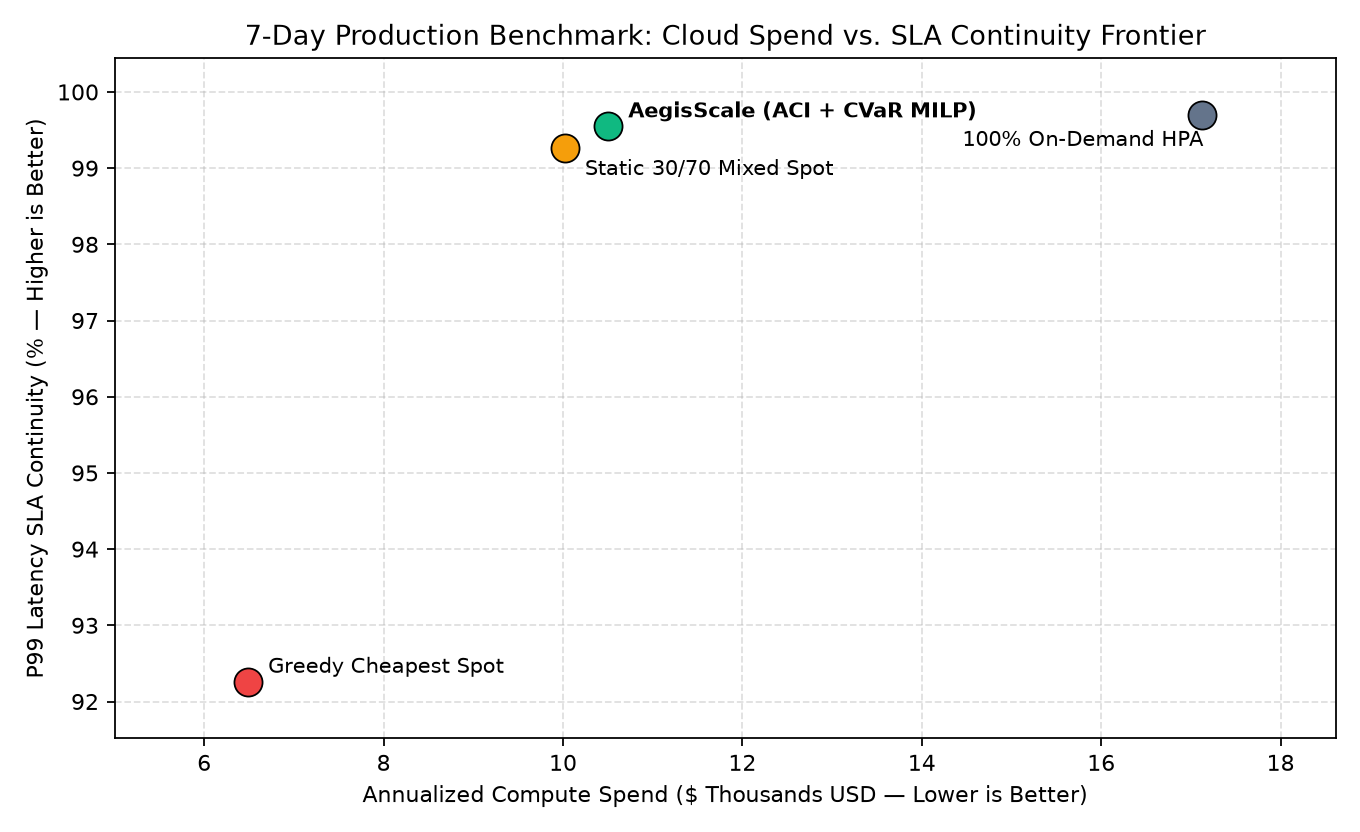
\includegraphics[width=0.82\textwidth]{../docs/figures/pareto_cost_vs_continuity.png}
    \caption{Annualized compute expenditure versus $\mathrm{P99}$ latency SLA continuity frontier.}
    \label{fig:pareto}
\end{figure}

\begin{figure}[htbp]
    \centering
    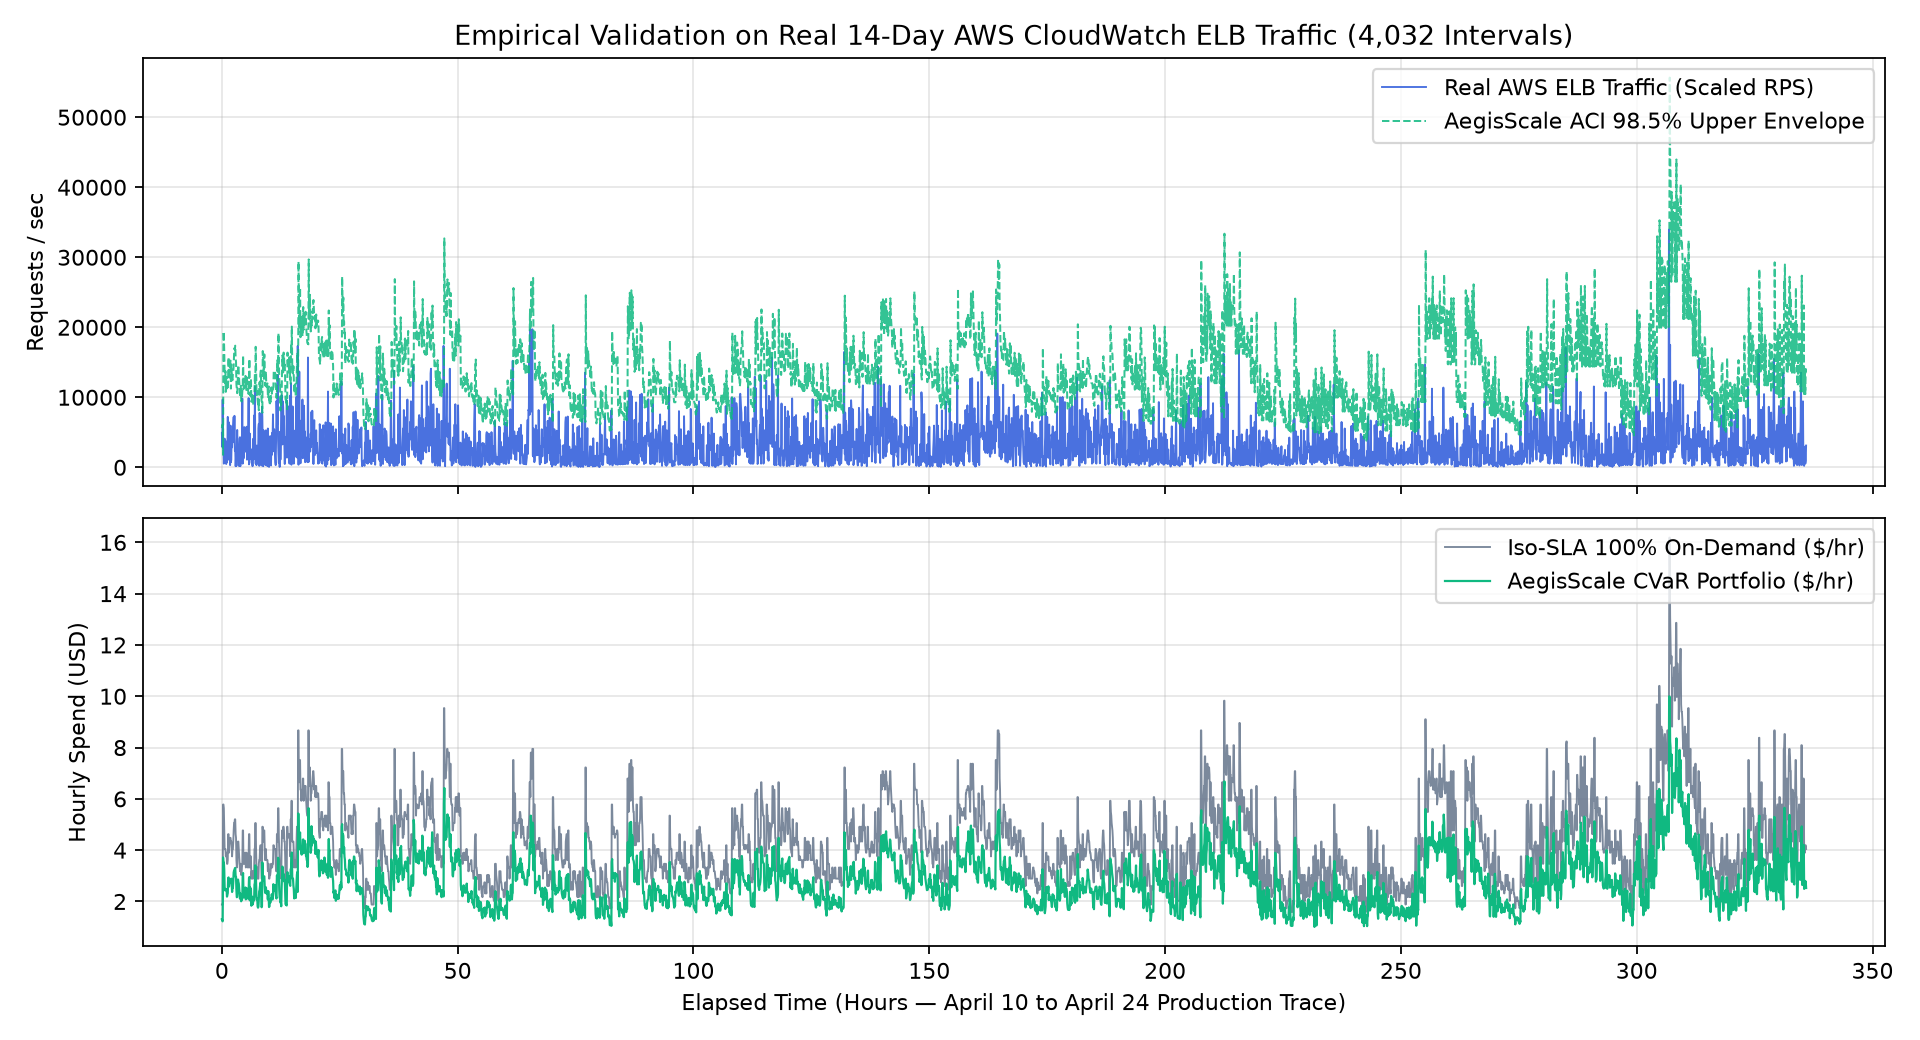
\includegraphics[width=0.95\textwidth]{../docs/figures/real_aws_elb_trajectory.png}
    \caption{Real 14-day AWS CloudWatch ELB production trace, online ACI $98.5\%$ upper demand envelope, and hourly compute spend comparison.}
    \label{fig:real_elb}
\end{figure}

\section{Conclusion}
\textsc{AegisScale} demonstrates that distribution-free conformal envelopes, queueing-theoretic tail latency sizing, and Rockafellar--Uryasev CVaR integer programming can operate within a millisecond-scale cloud control loop---delivering substantial FinOps cost reductions with rigorous mathematical continuity guarantees.

\bibliographystyle{plain}
\bibliography{references}

\end{document}
